\chapter{Berechnung der Systemeigenschaften}
\label{chap4}
Ziel dieser Arbeit soll der Vergleich verschiedener Kombinationen von Ladesystem und Speichertechnologie aus technischer Sicht ein. Qualitative Bewertungen einer Kombination sind teilweise ohne Rechnung möglich (z. B. "`\textsc{Primove} ist besser für Lithium-Titanat-Batterien geeignet als für Lithium-Eisenphosphat-Batterien"'). Eine genauere Betrachtung und ein Vergleich von ähnlichen Technologiekombinationen ist jedoch nicht möglich. Daher werden in dieser Arbeit mit Hilfe eines Simulationsmodell quantitative Daten zu den verschiedenen Technologiekombinationen ermittelt.

\section{Simulationsmodell}
\marginpar{Gibt es dazu ne Quelle?} Ausgangspunkt ist das existierende Elektrobus-Simulationsmodell des Fachgebiets MPM der TU Berlin. Dieses Modell ermittelt aus einer aufgezeichneten Busstrecke sowie Busparametern und Naturkonstanten den Energieverbrauch des Busses auf dieser Strecke. Sowohl die nötige Antriebsenergie als auch die rekuperierbare Bremsenergie werden berechnet.

Im Modell existierte nur eine Simulation für Lithium-Titanat-Batterien. Sie entspricht dem empirischen Model von Lam und Bauer \cite{lam2011practical}. Dieses Modell stellt eine Lithium-Titanat-batterie\marginpar{LiFePO?} in hoher Qualität dar, ist jedoch für andere Batterietypen ungeeignet. Daher wird für andere Batterietypen ein Modell nach Tremblay und Dessaint verwendet \cite{tremblay2009experimental}. Dieses Modell liefert weniger exakte Daten, kann aber dafür verschiedene Batterietypen darstellen. Die Batterie ist aus mehreren Zellen zusammengesetzt\footnote{Diese Zellen entsprechen nicht unbedingt einer chemischen Batteriezelle, sondern der kleinsten Batterie, die einzeln verfügbar ist.}. Das Modell berechnet die kleinste Zellenzahl, die nötig ist um die Strecke mit einer definierbaren Reserve zu durchfahren.

Die Ladezeit ist im Modell durch die aufgezeichnete Strecke festgelegt. Da in dieser Arbeit die Ladezeiten verschiedener Technologiekombinationen verglichen werden sollen, wurde ein separates Modell für den Ladevorgang erstellt. Es besteht aus der Batterie und einer Energiequelle, die nach einer Totzeit die maximale Ladeleistung bereitstellt. Die Batterie nimmt entsprechend ihrer Ladekurve diese Leistung teilweise oder vollständig auf. Wenn die Batterie den gewünschten Ladezustand erreicht hat, endet die Simulation und die gewünschten Ergebnisse können entnommen werden.

In Abbildung \ref{abb_sim} ist sind die Komponenten der Simulation als Flussdiagramm dargestellt.

\begin{figure}\centering
	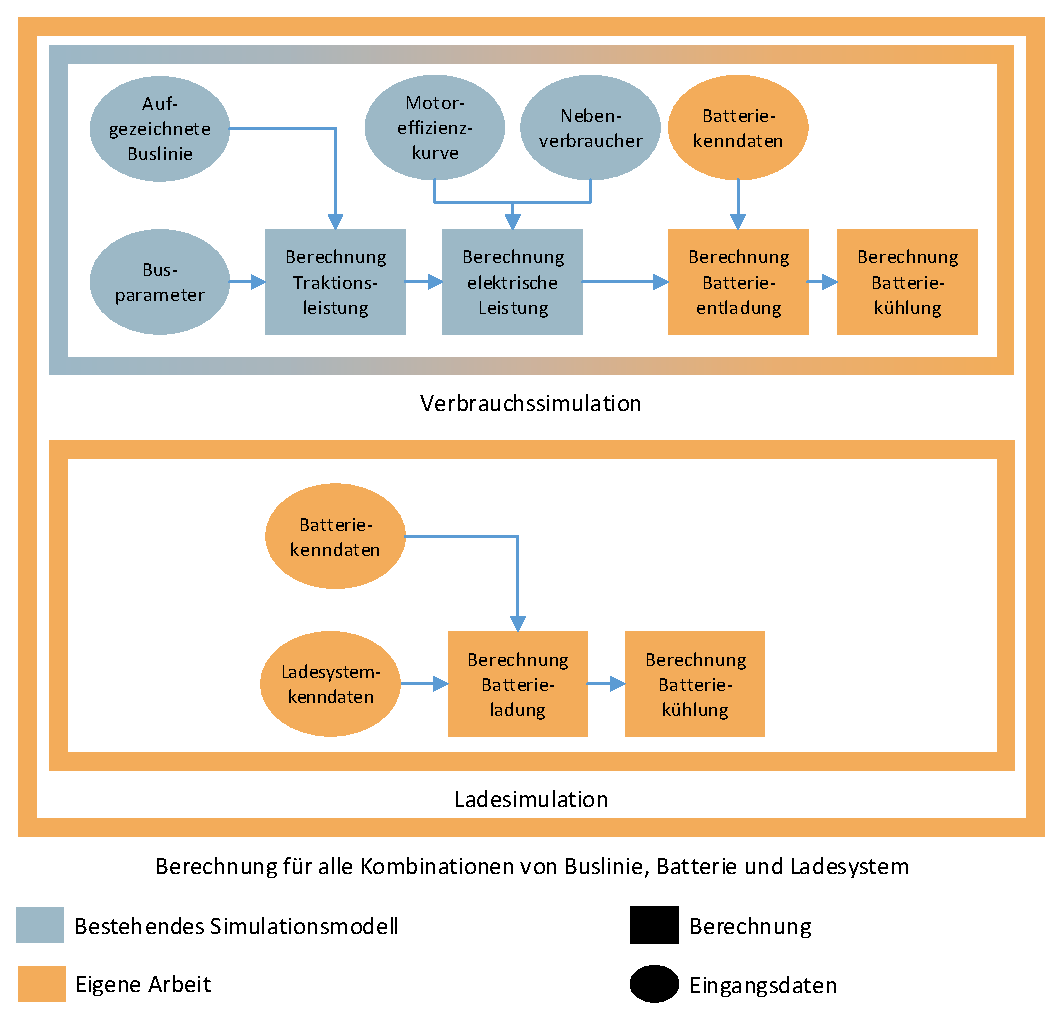
\includegraphics[height=19cm]{Simulation-Schaubild}
	\caption[Flussdiagramm der Simulation]{Flussdiagramm der Simulation. Parallelogramme stellen Eingabedaten da, Rechtecke Prozesse. Rauten sind Ausgabedaten, orangene Rauten fließen in die Bewertung der Kombination ein. der \emph{orangene Pfeil}  zeigt die kreisförmige Abhängigkeit von Batteriemasse und Energieverbrauch.}
	\label{abb_sim}
\end{figure}

\subsection{Verbrauchsrechung}
Die Verbrauchsrechnung berechnet den Energieverbrauch des Antriebsstrangs auf einer bestimmten Strecke.

Nebenverbraucher wie die Klimatisierung des Busses, Scheinwerfer, Druckluft etc. werden in dieses Simulation ausgeblendet. Sie sind unabhängig von Ladesystem und Speichertechnologie und von daher irrelevant für den Vergleich der Kombinationen.

\subsubsection{Eingabedaten}
\begin{description}
	\item[Fahrstrecke] Die Fahrstrecke des Bussem bestehend aus Zeit, Geschwindigkeit und Passagierzahl. Beschleunigung und Strecke werden durch Differenzieren bzw. Integrieren der Geschwindigkeit bestimmt, nicht durch die direkt gemessene Strecke.
	\item[Busparameter] Wirkungsrade für Antrieb und Rekuperation, Roll- und Luftwiderstände und Fahrzeugmasse.
	\item[Batteriemasse] \emph{Wird vom Speichersystem berechnet.} Gesamtmasse der Batterie.\marginpar{fehlt}
	\item[Ladesystemmasse] Gesamtmasse der busseitigen Komponenten des Ladesystems.
\end{description}

\subsubsection{Ausgabedaten}
\begin{description}
	\item[Energieverbrauch] Gesamtenergieverbrauch von Beginn der Strecke bis zum  Zeitpunkt \emph{t}.
	\item[Leistungsprofil] Die zum Zeitpunkt \emph{t} geforderte Leistung. Der Wert kann positiv oder negativ sein. Die Batterie \emph{muss} die geforderte (positive) Traktionsleistung liefern, sie \emph{kann} die durch Rekuperation bereitgestellte (negative) Leistung bis zu ihrere maximalen Ladeleistung ausnutzen. Darüber hinausgehende Rekuperationsleistung wird in den Bremswiderständen in Hitze umgesetzt.
\end{description}

\subsection{Speichersystem}
Das Speichersystem simuliert den Energiespeicher. Es kann eine bestimmte Energie (Einheit: $kWh$) speichern und abhängig vom Ladezustand eine begrenzte Leistung bereitstellen oder aufnehmen. Die Größe der Batterie wird durch eine Optimierung bestimmt. Intern besteht das Batteriemodell aus einer bestimmten Anzahl von Unterbatterien, die in Reihe oder parallel geschaltet sein können. Diese Unterbatterien können sowohl einzelne Zellen oder Batteriepacks sein.

\subsubsection{Eingabedaten}
\begin{description}
	\item[Leistungsprofil] Die Energie, die das Speichersystem liefern muss. Die Spitzenleistung ist das Maximum des Leistungsprofils, die Energie ergibt sich durch integrieren und die Durchschnittsleistung durch Division der Energie durch die Zeit. 
	\item[Parameter Unterbatterie] Gewicht, Volumen, Spannungskurven für verschiedene Ströme.
\end{description}

\subsubsection{Optimierung}
Mithilfe der Optimierung soll die kleinste Batterie gefunden werden, die auf dieser Strecke verwendet werden kann. Als zu minimierende Kriterien können also austauschbar Anzahl der Unterbatterien, Masse, Energie und Volumen verwendet werden.
\paragraph{Beschränkungen}
\begin{itemize}
	\item Pulsleistung
	\item Dauerleistung
	\item Ladezustand zu Beginn und Ende 
\end{itemize}

\subsubsection{Ausgabedaten}
\begin{description}
	\item[Batteriedaten] Gewicht und Größe der Batterie.
	\item[Batteriebeschränkungen] Die maximale Dauer- und Pulsladeleistung der Batterie
\end{description}

\subsection{Ladesystem}
Das Ladesystem modelliert den Ladevorgang, während der Bus an der Ladestation steht (dynamische Ladesysteme werden nicht berücksichtigt). Es erhält eine entladene Batterie und gibt eine aufgeladene Batterie sowie die verbrauchte Energie zurück.
Es wird angenommen, das die Stromrichter in Ladesystem und fahrzeugseitiger Ladeelektrik Spannung und Strom immer an die gewünschte Ladekurve der Batterie anpassen können.

\subsubsection{Eingabedaten}
\begin{description}
	\item[Ladekurve Batterie] Die Ladeleistung, die die Batterie bei einem bestimmten Ladezustand aufnehmen kann.
	\item[Zustand der Batterie] Ladezustand der Batterie zu Beginn des Ladevorgangs.
	\item[Spezifikation Ladesystem] Maximale Ladeleistung, Effizienz, Totzeiten.
\end{description}

\subsubsection{Ausgabedaten}
\begin{description}
	\item[Zustand der Batterie] Ladezustand der Batterie zum Ende des Ladevorgangs.
	\item[Energieverbrauch] Energieverbrauch des Ladesystems.
	\item[Zeitdauer] Dauer des Ladevorgangs.
\end{description}

\subsection{Kombination}

\subsubsection{Eingabedaten}
\begin{description}
	\item[Ladestrategie] Die verwendete Ladestrategie. Dies beeinflusst die Anzahl Fahrzyklen, bevor geladen wird. \emph{Oder gehört das zum Ladesystem?}
\end{description}

\subsubsection{Ausgabedaten}
\begin{description}
	\item[Effizienz] Definiert als das Verhältnis zwischen Energieverbrauch des Motors (aus der \emph{Verbrauchsrechnung}) und der aus dem Stromnetz entnommenen Energie (aus dem \emph{Ladeysytem}).
	\item[Anteil Ladezeit] Die Ladezeit pro Betriebsstunde. \emph{Oder die Fahrstunden, die man pro Ladestunde kriegt?}
	\item[Ladezyklen pro Kilometer] Wichtig für die Abschätzung der Lebensdauer.
\end{description}

\section{Ergebnisse}